%%This is a very basic article template.
%%There is just one section and two subsections.
\documentclass{article}
\usepackage{tkz-berge}
\usepackage{amsmath}

\title{Numeric simulation of a bubble mass}
\author{Tommaso Sciortino}
\date{October 2011}

\begin{document}
\maketitle
\section{Representation}
The bubble mass is represented by a graph: each edge represents a bubble wall;
each vertex the point where multiple bubble walls meet; each bubble a face. As
this is a 2D model the graph is planar. Since more than one wall may connect the same
two vertices the graph is a multigraph. Furthermore since only vertices where
three walls meet are physically stable we will contrain the graph to be
3-regular or ``cubic''. Similarly, loops are physically
unstable and thus disallowed.
\begin{figure}[h]
\centering
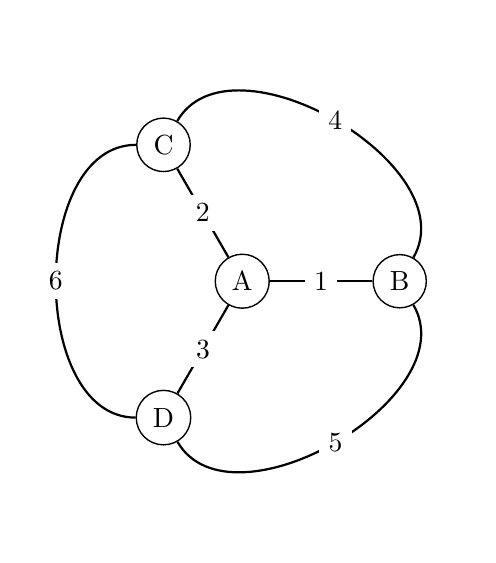
\begin{tikzpicture}[]
\GraphInit[vstyle=Normal] 
\Vertex[]{A}  
\Vertex[a=0, d=2cm]{B} 
\Vertex[a=120, d=2cm]{C}
\Vertex[a=240, d=2cm]{D} 
\Edge[label={1}](A)(B)
\Edge[label={2}](A)(C)
\Edge[label={3}](A)(D)
\Edge[style={bend left=90}, label={4}](C)(B)
\Edge[style={bend left=90}, label={5}](B)(D)
\Edge[style={bend left=90}, label={6}](D)(C) 
\end{tikzpicture}
\caption{A planar cubic graph}
\end{figure}

\subsection{Bubble as faces}
Each bubble is represented by a graph face; a ring of serially connected edges.
Each edge belongs to two faces: one for each of the two bubbles it forms the
border between. In addition to the normal internal faces there is one
``external'' unbounded face which will require special handling later on. It
represents the air outside the bubble mass.

If we imagine each edge to represent two directed edges (one in each direction)
then each face is a list of directed edges the head of each being
the tail of the next. Consequently, each directed edge belongs to exactly one
face. Except for the external face, the directed
edges in a face all run clockwise \begin{figure}[h]
\centering
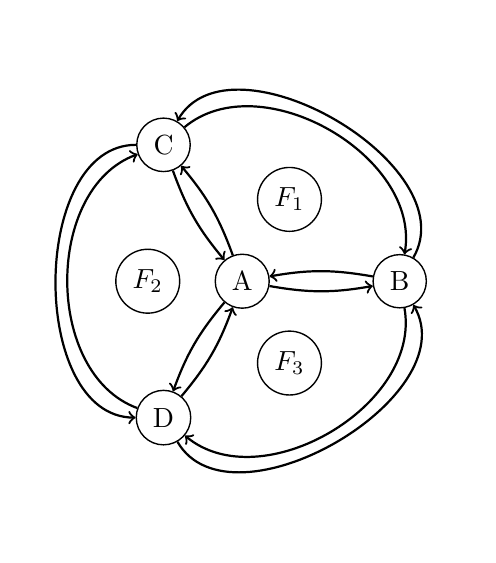
\begin{tikzpicture}[]
\GraphInit[vstyle=Normal] 
\Vertex[]{A}  
\Vertex[a=0, d=2cm]{B} 
\Vertex[a=120, d=2cm]{C}
\Vertex[a=240, d=2cm]{D} 
\Vertex[Math, a=60, d=1.2cm]{F_1}
\Vertex[Math, a=180, d=1.2cm]{F_2}
\Vertex[Math, a=300, d=1.2cm]{F_3} 
\Edge[style={<-,bend left=10}](A)(B)
\Edge[style={->,bend right=10}](A)(B)
\Edge[style={<-,bend left=10}](A)(C)
\Edge[style={->,bend right=10}](A)(C)
\Edge[style={<-,bend left=10}](A)(D)
\Edge[style={->,bend right=10}](A)(D)
\Edge[style={<-,bend left=90}](C)(B)
\Edge[style={->,bend left=70}](C)(B)
\Edge[style={<-,bend left=90}](B)(D)
\Edge[style={->,bend left=70}](B)(D)
\Edge[style={<-,bend left=90}](D)(C)
\Edge[style={->,bend left=70}](D)(C) 
\end{tikzpicture}
\caption{A directed graph representation}
\end{figure}
\subsection{Bubble walls as cubic beziers}
The position of a bubble wall is represented by a cubic bezier curve defined as
a parametric equation with four control points $\vec{B_n}(t)$
\begin{displaymath}
\vec{B}(p,t)=(1-p)^3\vec{B_0}(t)+3p(1-p)^2\vec{B_1}(t)+3p^2(1-p)\vec{B_2}(t)+p^3\vec{B_3}(t)
\end{displaymath}
The parameter p runs from 0 to 1. We also define
\begin{align*}
\vec{B}(p,t)&=B_x(p,t)\hat{x} +B_y(p,t)\hat{y}
\end{align*}
and
\begin{align*}
B_x(p,t)&=(1-p)^3x_0(t)+3p(1-p)^2x_1(t)+3p^2(1-p)x_2(t)+p^3x_3(t)\\
B_y(p,t)&=(1-p)^3y_0(t)+3p(1-p)^2y_1(t)+3p^2(1-p)y_2(t)+p^3y_3(t)
\end{align*}
\section{Physics}
To derive equations of motion we use the Euler-Lagrange equation. The Lagrangian
$\mathcal{L}_T=K_T-V_T$ is the total kinetic minus total potential energy of the
system. $\mathcal{L}_T$ is defined in terms of $q_i,\dots,q_n$, the generalized coordinates
which completely describe the state of the system at time $t$. (In our case these are the
functions of time describing the positions of the control points
for all bubble walls.) For each one we derive the equation:
\begin{align*}
\frac{d}{d t}\frac{\partial \mathcal{L}_T}{\partial q'_i}
=\frac{\partial
\mathcal{L}_T}{\partial q_i} 
\end{align*} 
Taken together these yield a nonlinear system of ordinary differential
equations. We cannot solve these in closed form but we can approximate a numeric solution.
\subsection{Kinetic Energy}
To find the kinetic energy we must determine the velocity of every point on a
bubble wall. To do this we take the derivative of the position with respect to
time.
\begin{displaymath}
\vec{B}'(p,t)=(1-p)^3\vec{B_0}'(t)+3p(1-p)^2\vec{B_1}'(t)+3p^2(1-p)\vec{B_2}'(t)+p^3\vec{B_3}'(t)
\end{displaymath}
To have Kinetic enegery the wall must have mass so we introduce a coefficient
$m$ to represent mass per unit length of p. This gives us the kinetic energy at the
infintesimal point p
\begin{displaymath}
K(p,t) = \frac{m}{2} \left|\vec{B}'(p,t)\right|^2
\end{displaymath}
To find the total kinetic energy for the bubble wall we integrate over the
length of the wall
\begin{align*}
K(t)&= \int_0^1 \frac{m}{2} \left|\vec{B}'(p,t)\right|^2 dp\\
&=\frac{m}{2} \int_0^1 \left(\sqrt{B'_x(p,t)^2+B'_y(p,t)^2}\right)^2 dp\\
&=\frac{m}{2} \int_0^1 B'_x(p,t)^2+B'_y(p,t)^2 dp
\end{align*}
In terms of the derivatives of the coordinates of the 4 control points $x_n(t)$
and $y_n(t)$ we get:
\begin{align*}
K(t)=\frac{m}{2} \int_0^1
\left((1-p)^3x'_0+3p(1-p)^2x'_1+3p^2(1-p)x_2'+p^3x'_3\right)^2 \\
 \quad+ \left((1-p)^3y'_0+3p(1-p)^2y'_1+3p^2(1-p)y'_2+p^3y'_3
\right)^2 dp
\end{align*}
Integrating gives us
\begin{align*}
K(t)=\frac{m}{2} &\left( 
\frac{x_0^{'2}}{7} + \frac{x'_0 x'_1}{7} + \frac{2 x'_0 x'_2}{35} + 
\frac{x'_0 x'_3}{70}  + \frac{3 x_1^{'2}}{35} \right.\\
&\left.\quad +\frac{9 x'_1 x'_2}{70} 
+ \frac{2 x'_1 x'_3}{35} + \frac{3 x_2^{'2}}{35} + \frac{x'_2 x'_3}{7} +\frac{x_3^{'2}}{7}\right.\\
&\quad\left. +\frac{y_0^{'2}}{7} + \frac{y'_0 y'_1}{7} + \frac{2 y'_0 y'_2}{35} + 
\frac{y'_0 x'_3}{70} + \frac{3 y_1^{'2}}{35} \right.\\
&\left.\quad  +\frac{9 y'_1 y'_2}{70} 
+ \frac{2 y'_1 y'_3}{35} + \frac{3 y_2^{'2}}{35} + \frac{y'_2 y'_3}{7}
+\frac{y_3^{'2}}{7}\right)
\end{align*}
Rephrased more clearly (possibly) with matrices:
\begin{align*}
K(t)=
\frac{m}{140} &\left(
\begin{bmatrix} x'_0 & x'_1 & x'_2 & x'_3 \end{bmatrix}
 \begin{bmatrix} 
10 & 10 & 4 & 1\\
0 & 6 & 9 & 4\\
0 & 0 & 6 & 10\\
0 & 0 & 0 & 10\\ 
\end{bmatrix}
\begin{bmatrix} x'_0\\x'_1\\x'_2\\x'_3 \end{bmatrix}
\right.\\
&+ \left.
\begin{bmatrix} y'_0 & y'_1 & y'_2 & y'_3 \end{bmatrix}
 \begin{bmatrix} 
10 & 10 & 4 & 1\\
0 & 6 & 9 & 4\\
0 & 0 & 6 & 10\\
0 & 0 & 0 & 10\\ 
\end{bmatrix}
\begin{bmatrix} y'_0\\y'_1\\y'_2\\y'_3 \end{bmatrix} 
\right)
\end{align*}
Note that $K$ is just for one bubble wall. To get the total
kinetic energy of the system $K_T$ we must sum the kinetic energy of all the
walls. Note too that each bezier curve end point is shared by three walls. This
means the some cooridnates $x_n, y_n$ will appear in more than one wall's kinetic energy equation.
\subsection{Potential Energy}
Potential energy in our system comes from two sources, air pressure and surface
tension. Surface tension potential rises as a wall lengthens.
Air pressure potential rises as the air inside a bubble is compressed.
\subsubsection{Air Pressure Potential}
We use the ideal gas law to estimate the
behavior of the gas in the bubble under pressure. Here $P(t)$ and $A(t)$ are
pressure and area of the bubble, $T$ the temperature, $N$ the number of particles in the
gas, and $k$ is Boltzmann's constant (modified for 2 dimensions). We will assume
that all processes are isothermal and that $N$ is constant.
\begin{align*}
P(t)=\frac{NkT}{A(t)}=\frac{constant}{A(t)}
\end{align*}
The energy neccessary to change a bubble's area from $A_1$ to $A_2$ is
\begin{align*}
\Delta E = \int_{A_1}^{A_2} P dA = \int_{A_1}^{A_2} \frac{NkT}{A} dA = NkT
\ln\left(\frac{A_2}{A_1}\right)
\end{align*}
We define the ``ambient'' pressure of the outside air and $\rho$ and $A_\rho$ as
the area of the bubble when at this pressure. Then the energy stored as
potential in a bubble of area $A(t)$ is
\begin{align*}
V_p(t) = -\rho A_\rho \ln\left(\frac{A(t)}{A_\rho}\right) = \rho A_\rho
\ln\left(\frac{A_\rho}{A(t)}\right)
\end{align*}

Though the above formula works for normal bubbles, we must deal seperately with
the open air outside the bubble mass (represented by the unbounded face). Since
the area of this bubble is infinite the formula will not apply directly.
However, if we imagine the bubble mass is floating in a large (but finite!) room
and then take the limit as the room because infinitly large we can get a formula
for the energy. Let $A_r$ be the area of the room and $A_m$ be the area of the
bubble mass. Then the area of the extrnal bubble is $A_r-A_m$ and the energy
required to go from $A_r$ to $A_r-A_m$ is
\begin{align*}
V_p(t) = \lim_{A_r\to\infty} \rho A_r \ln\left(\frac{A_r}{A_r-A_m(t)}\right)=
\rho A_m(t)
\end{align*}

All that remains is to determine the area of the bubble. This is simply the sum
of the signed area under the curves that make it up. The formula for the area
under a bezier curve is
\begin{align*}
A_b &= \int_0^1 B_y(p)\frac{\partial B_x(p)}{dp} dp\\
&=\int_0^1
\left((1-p)^3y_0+3p(1-p)^2y_1+3p^2(1-p)y_2+p^3y_3\right)\\
&\quad \left(-3(1-p)^2x_0 +3(1+p(3p-4))x_1+3p(2-3p)x_2 +3p^2x_3\right)dp\\
&= x_0\left( \frac{-y_0}{2}+ \frac{-3y_1}{10}+\frac{-3y_2}{20}+\frac{-y_3}{20}\right)\\
&+ x_1\left(\frac{3y_0}{10}+ \frac{-3y_2}{20} +\frac{-3y_3}{20}\right)\\
&+ x_2\left(\frac{3y_0}{20}+ \frac{3y_1}{20} +\frac{-3y_3}{10}\right)\\
&+ x_3\left(\frac{y_0}{20} + \frac{3y_1}{20} +\frac{3y_2}{10}
+\frac{y3}{2}\right)
\end{align*}
Rephrased more succinctly with matrices:
\begin{align*}
A_b=
\frac{1}{20} 
\begin{bmatrix} x_0 & x_1 & x_2 & x_3 \end{bmatrix}
\begin{bmatrix} 
-10 & -6 & -3 & -1\\
6 & 0 & -3 & -3\\
3 & 3 & 0 & -6\\
1 & 3 & 6 & 10\\ 
\end{bmatrix}
\left[ \begin{array}{c} y_0\\y_1\\y_2\\y_3 \end{array} \right] 
\end{align*}
Special care should be taken when calculating the area of a bubble to ensure
that the area under the curve is being calculated in the correct direction.
The area under the curve from $\vec{B_0}$ to $\vec{B_3}$ has the opposite sign
of that from $\vec{B_3}$ to $\vec{B_1}$.

Of course to get the total potential due to pressure you need to sum all walls
of all bubbles in the mass.
\subsubsection{Surface Tension Potential}
The potential energy due to surface tension varies linearly with wall length. We
will introduce a coefficient $\tau$ for energy per unit length.
\begin{align*}
V_s(t)&=\tau Length(B)\\
&=\tau \int_0^1 \left|\frac{d \vec{B}(p,t)}{dp}\right| dp\\
&=\tau \int_0^1 \sqrt{\left(\frac{d B_x(p,t)}{dp}\right)^2+\left(\frac{d
B_y(p,t)}{dp}\right)^2} dp
\end{align*}
where
\begin{align*}
\frac{d B_x(p,t)}{dp}&= -3(1-p)^2x_0 +3(3p-1) (p-1)x_1+3p(2-3p)x_2 +3p^2x_3\\
\frac{d B_y(p,t)}{dp}&= -3(1-p)^2y_0 +3(3p-1) (p-1)y_1+3p(2-3p)y_2 +3p^2y_3
\end{align*}
Since the value in the square root is a 4th degree polynomial in p this
integral cannot generally be solved in closed form.
\subsection{Calculating the equations of motion}
Having calulated the kinetic and potential energy of the system we can finally
apply use them to calculate the Lagrangian $\mathcal{L}_T=K_T-V_T$.

Observe that the formula for kinetic energy is defined only in terms of
the velocities of the control points ($q'_1,\dots,q'_n$) and the potential is
defined only in terms of positions of the control points ($q_1,\dots,q_n$).
This simplifies the equations of motion greatly
\begin{align*}
\frac{d}{d t}\frac{\partial \mathcal{L}_T}{\partial q'_n} 
&=\frac{\partial \mathcal{L}_T}{\partial q} \\
\frac{d}{d t}\frac{\partial (K_T-V_T)}{\partial q'_n}
&= \frac{\partial (K_T-V_T)}{\partial q} \\
\frac{d}{d t}\left( \frac{\partial K_T}{\partial q'_n} - \frac{\partial
V_T}{\partial q'_n}\right)
&=\frac{\partial K_T}{\partial q}-\frac{\partial V_T}{\partial q} \\
\frac{d}{d t} \frac{\partial K_T}{\partial q'_n}
&=-\frac{\partial V_T}{\partial q}\\
\frac{d}{d t} \frac{\partial K_T}{\partial q'_n}
&= -\left(\frac{\partial V_{Tp}}{\partial q_n}+\frac{\partial V_{Ts}}{\partial
q_n}\right)
\end{align*}
To get the equations of motion we need to calculate the above equation for every
control point coordinate in the system. This means generating 8 equations for
every bubble wall in the system. We will only work out 2 such equations here as
the rest can be inferred from them by symmetry.
\subsubsection{Second Control Point}
We will generate the the lagrangian for the x coordinate of the second control
point of the bubble wall. This case is simpler than the first coordinate which
is shared by three walls. Our equation is thus
\begin{align*}
 \frac{d}{d t} \frac{\partial K_T}{\partial x'_1} =-\left(\frac{\partial
 V_{Ts}}{\partial x_1} + \frac{\partial V_{Tp}}{\partial x_1}\right)
\end{align*}

First observe that since $x_1$ only appears in the kinetic energy formula for
one wall the quantity $\frac{\partial K_T}{\partial x'_1}=\frac{\partial K}{\partial x'_1}$
 so the left hand side of the lagrangian equation is 
\begin{align*}
\frac{d}{d t} \frac{\partial K_T}{\partial x'_1} &=
\frac{d}{d t} \frac{\partial K}{\partial x'_1}\\
 &= \frac{d}{d t}
 \frac{\partial }{\partial x'_1} \frac{m}{140} \left(
\begin{bmatrix} x'_0 & x'_1 & x'_2 & x'_3 \end{bmatrix}
 \begin{bmatrix} 
10 & 10 & 4 & 1\\
0 & 6 & 9 & 4\\
0 & 0 & 6 & 10\\
0 & 0 & 0 & 10\\ 
\end{bmatrix}
\begin{bmatrix} x'_0\\x'_1\\x'_2\\x'_3 \end{bmatrix}
\right.\\
&\qquad\qquad\qquad+ \left.
\begin{bmatrix} y'_0 & y'_1 & y'_2 & y'_3 \end{bmatrix}
 \begin{bmatrix} 
10 & 10 & 4 & 1\\
0 & 6 & 9 & 4\\
0 & 0 & 6 & 10\\
0 & 0 & 0 & 10\\ 
\end{bmatrix}
\begin{bmatrix} y'_0\\y'_1\\y'_2\\y'_3 \end{bmatrix} 
\right)\\ 
&= \frac{m}{140} \frac{d}{d t}\left(10x'_0+12x'_1+9x'_2+4x'_3 \right)\\
&= \frac{m}{140} \left(10x''_0+12x''_1+9x''_2+4x''_3 \right)
\end{align*}

The right side has two parts. One for pressure and one for surface tension. We
calculate the presure part first. 

Observe that $x_1$ only appears in the formula for the areas of the bubbles
$A_1$ and $A_2$ on either side of the bubble wall. Let $A_{1\rho}$ and
$A_{2\rho}$ be their area at ambient pressure. 
\begin{align*}
\frac{\partial V_{Tp}}{\partial x_1} &= \frac{\partial }{\partial x_1}
\left(
\rho A_{1\rho}
\ln\left(\frac{A_{1\rho}}{A_1}\right)
+\rho A_{2\rho}
\ln\left(\frac{A_{2\rho}}{A_2}\right)
\right)\\
&= 
\rho \left(
\frac{A_{1\rho}}{A_1} \frac{\partial A_1}{\partial x_1}
+\frac{A_{2\rho}}{A_2} \frac{\partial A_2}{\partial x_1}
\right)
\end{align*}
A tricky observation: The wall is oriented left-to-right in one bubble and
right-to-left in another. This introduces a sign change n one of them (I'll
arbitrarily choose $A_2$).
\begin{align*}
\frac{\partial V_{Tp}}{\partial x_1} &= 
\rho \left(
\frac{A_{1\rho}}{A_1} \frac{3}{20}(2y_0-y_2-y_3)
-\frac{A_{2\rho}}{A_2} \frac{3}{20}(2y_0-y_2-y_3)
\right)\\
&= 
 \frac{3\rho}{20} (2y_0-y_2-y_3)
\left( \frac{A_{1\rho}}{A_1} -\frac{A_{2\rho}}{A_2}\right)
\end{align*}
Lastly, observe that if one of the bubbles is the ``outside air'' it's factor
$\frac{A_{\rho}}{A}$ is 1.

Finally we get to the surface tension. Unfortunately there's not much that can
be done to simplify this expression as it's integral is unreducable.
\begin{align*}
\frac{\partial V_s(t)}{\partial x_1}&=
\frac{\partial}{\partial x_1}
\tau \int_0^1 \sqrt{\left(\frac{d B_x(p,t)}{dp}\right)^2+\left(\frac{d
B_y(p,t)}{dp}\right)^2} dp\\
&=
\tau\int_0^1\frac{\left(\frac{\partial}{\partial x_1}\frac{d
B_x(p,t)}{dp}\right) \frac{d B_x(p,t)}{dp}}{
  \sqrt{\left(\frac{d B_x(p,t)}{dp}\right)^2+\left(\frac{d
B_y(p,t)}{dp}\right)^2}} dp\\
&=
\tau\int_0^1\frac{3(3p-1)(p-1))  \frac{d B_x(p,t)}{dp}}{
  \sqrt{\left(\frac{d B_x(p,t)}{dp}\right)^2+\left(\frac{d
B_y(p,t)}{dp}\right)^2}} dp
\end{align*}
This value must be calculated by numeric integration.

All together that gives us
\begin{align*}
\frac{m}{140} \left(10x''_0+12x''_1+9x''_2+4x''_3 \right) &= 
 \frac{3\rho}{20} (2y_0-y_2-y_3)
\left( \frac{A_{1\rho}}{A_1} -\frac{A_{2\rho}}{A_2}\right)\\
&+\tau\int_0^1\frac{3(3p-1)(p-1))  \frac{d B_x(p,t)}{dp}}{
  \sqrt{\left(\frac{d B_x(p,t)}{dp}\right)^2+\left(\frac{d
B_y(p,t)}{dp}\right)^2}} dp
\end{align*}
\subsection{First Control Point}
We will generate the the lagrangian for the x coordinate of a vertex ($x_0$);
the joint endpoints of three bubble walls. We shall use $\alpha$, $\beta$, and $\gamma$ to
distinguish the walls.

The left hand side of the lagrangian equation is 
\begin{align*}
\frac{d}{d t} \frac{\partial K_T}{\partial x'_0}&=
\frac{m}{140}  \left( 20x''_0+10x''_{1\alpha}+4x''_{2\alpha}+x''_{3\alpha} \right)\\
&\qquad\qquad +\frac{m}{140}\left(
20x''_0+10x''_{1\beta}+4x''_{2\beta}+x''_{3\beta}\right)\\ 
&\qquad\qquad +\frac{m}{140} \left(
20x''_0+10x''_{1\gamma}+4x''_{2\gamma}+x''_{3\gamma} \right)\\
 &=\frac{m}{140} \left(
60x''_0
+10(x''_{1\alpha}+x''_{1\beta}+x''_{1\gamma})\right.\\
&\qquad\qquad \left.+4(x''_{2\alpha}+x''_{2\beta}+x''_{2\gamma})
+(x''_{3\alpha}+x''_{3\beta}+x''_{3\gamma}) \right)
\end{align*}

For the pressure part of the right hand side of the lagrangian we will use
$A_{\alpha\beta}$ and so on to denote the bubble which shares walls $\alpha$ and
$\beta$

\begin{align*}
\frac{\partial V_{Tp}}{\partial x_1} &= 
\rho \left(
\frac{A_{\alpha\beta\rho}}{A_{\alpha\beta}} \frac{\partial
A_{\alpha\beta}}{\partial x_0} 
+\frac{A_{\beta\gamma\rho}}{A_{\beta\gamma}} \frac{\partial
A_{\beta\gamma}}{\partial x_0} 
+\frac{A_{\gamma\alpha\rho}}{A_{\gamma\alpha}} \frac{\partial
A_{\gamma\alpha}}{\partial x_0} 
\right)
\end{align*}
Where
\begin{align*}
\frac{\partial A_{\alpha\beta}}{\partial x_0}=\frac{1}{20}
\left(-10(y_{0\alpha}+y_{0\beta})-6(y_{1\alpha}y_{1\beta})-3(y_{2\alpha}+y_{2\beta})-(y_{3\alpha}+y_{3\beta})\right)
\end{align*}

For the tension part of the right hand side we have
\begin{align*}
\frac{\partial V_s(t)}{\partial x_0}&=
\tau\left(\int_0^1\frac{3(1-p)^2  \frac{d B_{\alpha x}}{dp}}{
  \sqrt{\left(\frac{d B_{\alpha x}}{dp}\right)^2+\left(\frac{d
B_{\alpha y}}{dp}\right)^2}} dp\right.\\
&\qquad \left.+\int_0^1\frac{3(1-p)^2  \frac{d B_{\beta x}}{dp}}{
  \sqrt{\left(\frac{d B_{\beta x}}{dp}\right)^2+\left(\frac{d
B_{\beta y}}{dp}\right)^2}} dp\right.\\
&\qquad \left.+\int_0^1\frac{3(1-p)^2  \frac{d B_{\gamma x}}{dp}}{
  \sqrt{\left(\frac{d B_{\gamma x}}{dp}\right)^2+\left(\frac{d
B_{\gamma y}}{dp}\right)^2}} dp
\right)
\end{align*}

Putting this monstrosity together is left as an excersize to the reader.
\subsection{Solving the equations of motion}
We are now able to produce the equations of motion all that is left is to solve
them. Since the equations can't even be written in closed form it's
unsurprising that they can't be solved in closed form either. Instead we'll
use a slightly modified form of the ``forward Euler'' method for approximating
the solution to ODEs.

Observe that for every generalized coordinate $q_j$ we get one equation of the
form:
\begin{align*}
\sum_i^n c_{ij}q_i''(t) = F_j(q_1,q_2,\ldots)
\end{align*}
Here $c_{ij}$ is a coeficieint determined above and $F_j$ is
$-\frac{\partial V(t)}{\partial q_j}$.

If we may generalize $F_j$ to the matrix function $F$ these can be expressed in
matrix form:
\begin{align*}
C \vec{q''}= F \vec{q}
\end{align*}
Note that neither $C$ nor $F$ change unless the graph configuration changes.

Now all that is left is to numerically solve. We start with a initial positions
and velocities $\vec{q}$ and $\vec{q'}$. We use the above formula to determine
an aproximation for $\vec{q''}$, use that and the velocity to approximate the
location after elapsed time span $t$ and get a new set of $\vec{q}$ and
$\vec{q'}$. Repeat ad infinitum.
\section{Sources of Error}
For the sake of tractability I've choosen to represent a bubble wall with a
cubic bezier. Having only 8 degrees of freedom Cubic bezier curves cannot
represent all possible configurations for a deformed bubble wall. Even
worse, it cannot represent an arc of a circle which is the rest shape of a real
bubble wall.

\end{document}